\section{eo\-IBEAAvg\-Sorting$<$ EOT, Fitness\-Eval $>$ Class Template Reference}
\label{classeoIBEAAvgSorting}\index{eoIBEAAvgSorting@{eoIBEAAvgSorting}}
Functor The sorting phase of IBEA (Indicator-Based Evolutionary Algorithm) under uncertainty using averaged values for each objective Follow the idea presented in the Deb \& Gupta paper \char`\"{}Searching for Robust Pareto-Optimal Solutions in Multi-Objective Optimization\char`\"{}, 2005 Of course, the fitness of an individual needs to be an eo\-Stochastic\-Pareto\-Fitness object.  


{\tt \#include $<$eo\-IBEA.h$>$}

Inheritance diagram for eo\-IBEAAvg\-Sorting$<$ EOT, Fitness\-Eval $>$::\begin{figure}[H]
\begin{center}
\leavevmode
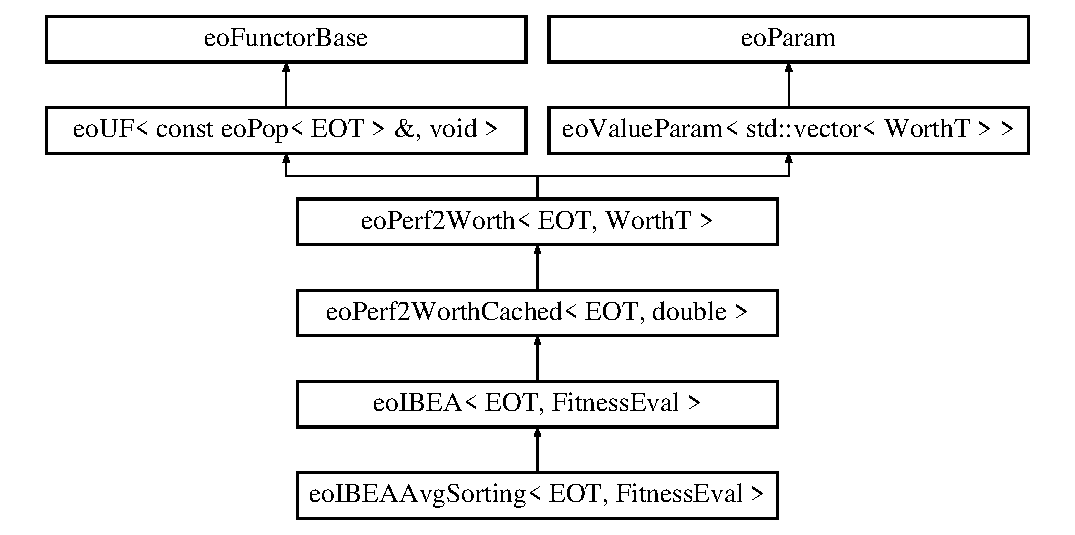
\includegraphics[height=6cm]{classeoIBEAAvgSorting}
\end{center}
\end{figure}
\subsection*{Public Member Functions}
\begin{CompactItemize}
\item 
{\bf eo\-IBEAAvg\-Sorting} ({\bf eo\-Binary\-Quality\-Indicator}$<$ Fitness\-Eval $>$ $\ast$\_\-I, const double \_\-kappa)
\begin{CompactList}\small\item\em constructor \item\end{CompactList}\end{CompactItemize}
\subsection*{Private Member Functions}
\begin{CompactItemize}
\item 
void {\bf set\-Bounds} (const {\bf eo\-Pop}$<$ EOT $>$ \&\_\-pop)
\begin{CompactList}\small\item\em computation and setting of the bounds for each objective \item\end{CompactList}\item 
void {\bf fitnesses} (const {\bf eo\-Pop}$<$ EOT $>$ \&\_\-pop)
\begin{CompactList}\small\item\em computation and setting of the fitness for each individual of the population \item\end{CompactList}\end{CompactItemize}
\subsection*{Private Attributes}
\begin{CompactItemize}
\item 
double {\bf kappa}\label{classeoIBEAAvgSorting_6f467d673861830d6a0708f61cecc3f7}

\begin{CompactList}\small\item\em scaling factor kappa \item\end{CompactList}\end{CompactItemize}


\subsection{Detailed Description}
\subsubsection*{template$<$class EOT, class Fitness\-Eval = typename EOT::Fitness::Fitness\-Eval$>$ class eo\-IBEAAvg\-Sorting$<$ EOT, Fitness\-Eval $>$}

Functor The sorting phase of IBEA (Indicator-Based Evolutionary Algorithm) under uncertainty using averaged values for each objective Follow the idea presented in the Deb \& Gupta paper \char`\"{}Searching for Robust Pareto-Optimal Solutions in Multi-Objective Optimization\char`\"{}, 2005 Of course, the fitness of an individual needs to be an eo\-Stochastic\-Pareto\-Fitness object. 



Definition at line 373 of file eo\-IBEA.h.

\subsection{Constructor \& Destructor Documentation}
\index{eoIBEAAvgSorting@{eo\-IBEAAvg\-Sorting}!eoIBEAAvgSorting@{eoIBEAAvgSorting}}
\index{eoIBEAAvgSorting@{eoIBEAAvgSorting}!eoIBEAAvgSorting@{eo\-IBEAAvg\-Sorting}}
\subsubsection{\setlength{\rightskip}{0pt plus 5cm}template$<$class EOT, class Fitness\-Eval = typename EOT::Fitness::Fitness\-Eval$>$ {\bf eo\-IBEAAvg\-Sorting}$<$ EOT, Fitness\-Eval $>$::{\bf eo\-IBEAAvg\-Sorting} ({\bf eo\-Binary\-Quality\-Indicator}$<$ Fitness\-Eval $>$ $\ast$ {\em \_\-I}, const double {\em \_\-kappa})\hspace{0.3cm}{\tt  [inline]}}\label{classeoIBEAAvgSorting_eb0cfda626e1e5cac6750f0598610f82}


constructor 

\begin{Desc}
\item[Parameters:]
\begin{description}
\item[{\em eo\-Binary\-Quality\-Indicator$<$EOT$>$$\ast$}]\_\-I the binary quality indicator to use in the selection process \item[{\em double}]\_\-kappa scaling factor kappa \end{description}
\end{Desc}


Definition at line 385 of file eo\-IBEA.h.

References eo\-IBEAAvg\-Sorting$<$ EOT, Fitness\-Eval $>$::kappa.

\subsection{Member Function Documentation}
\index{eoIBEAAvgSorting@{eo\-IBEAAvg\-Sorting}!setBounds@{setBounds}}
\index{setBounds@{setBounds}!eoIBEAAvgSorting@{eo\-IBEAAvg\-Sorting}}
\subsubsection{\setlength{\rightskip}{0pt plus 5cm}template$<$class EOT, class Fitness\-Eval = typename EOT::Fitness::Fitness\-Eval$>$ void {\bf eo\-IBEAAvg\-Sorting}$<$ EOT, Fitness\-Eval $>$::set\-Bounds (const {\bf eo\-Pop}$<$ EOT $>$ \& {\em \_\-pop})\hspace{0.3cm}{\tt  [inline, private, virtual]}}\label{classeoIBEAAvgSorting_b365a1eab0da5211c59369416642780d}


computation and setting of the bounds for each objective 

\begin{Desc}
\item[Parameters:]
\begin{description}
\item[{\em const}]eo\-Pop$<$EOT$>$\& \_\-pop the population \end{description}
\end{Desc}


Implements {\bf eo\-IBEA$<$ EOT, Fitness\-Eval $>$} {\rm (p.\,\pageref{classeoIBEA})}.

Definition at line 413 of file eo\-IBEA.h.\index{eoIBEAAvgSorting@{eo\-IBEAAvg\-Sorting}!fitnesses@{fitnesses}}
\index{fitnesses@{fitnesses}!eoIBEAAvgSorting@{eo\-IBEAAvg\-Sorting}}
\subsubsection{\setlength{\rightskip}{0pt plus 5cm}template$<$class EOT, class Fitness\-Eval = typename EOT::Fitness::Fitness\-Eval$>$ void {\bf eo\-IBEAAvg\-Sorting}$<$ EOT, Fitness\-Eval $>$::fitnesses (const {\bf eo\-Pop}$<$ EOT $>$ \& {\em \_\-pop})\hspace{0.3cm}{\tt  [inline, private, virtual]}}\label{classeoIBEAAvgSorting_4bc8c46d151d7935d7b2ac8bfbdd7ee6}


computation and setting of the fitness for each individual of the population 

\begin{Desc}
\item[Parameters:]
\begin{description}
\item[{\em const}]eo\-Pop$<$EOT$>$\& \_\-pop the population \end{description}
\end{Desc}


Implements {\bf eo\-IBEA$<$ EOT, Fitness\-Eval $>$} {\rm (p.\,\pageref{classeoIBEA})}.

Definition at line 445 of file eo\-IBEA.h.

The documentation for this class was generated from the following file:\begin{CompactItemize}
\item 
eo\-IBEA.h\end{CompactItemize}
